\section{Diagrammi riassuntivi dei \gl{package}}
Di seguito sono riportati tutti i package dell’applicativo per chiarire la relazione tra le componenti e le classi al suo interno. Per chiarezza ed esigenza di spazio le classi rappresentate all’interno dei package sono rappresentate senza metodi e attributi.


\subsection{Back-end}
\gl{Package} contenente tutte le componenti che costituiscono il back-end. Le componenti sono organizzate secondo il pattern a \gl{microservizi}.
\begin{figure}[h] \centering 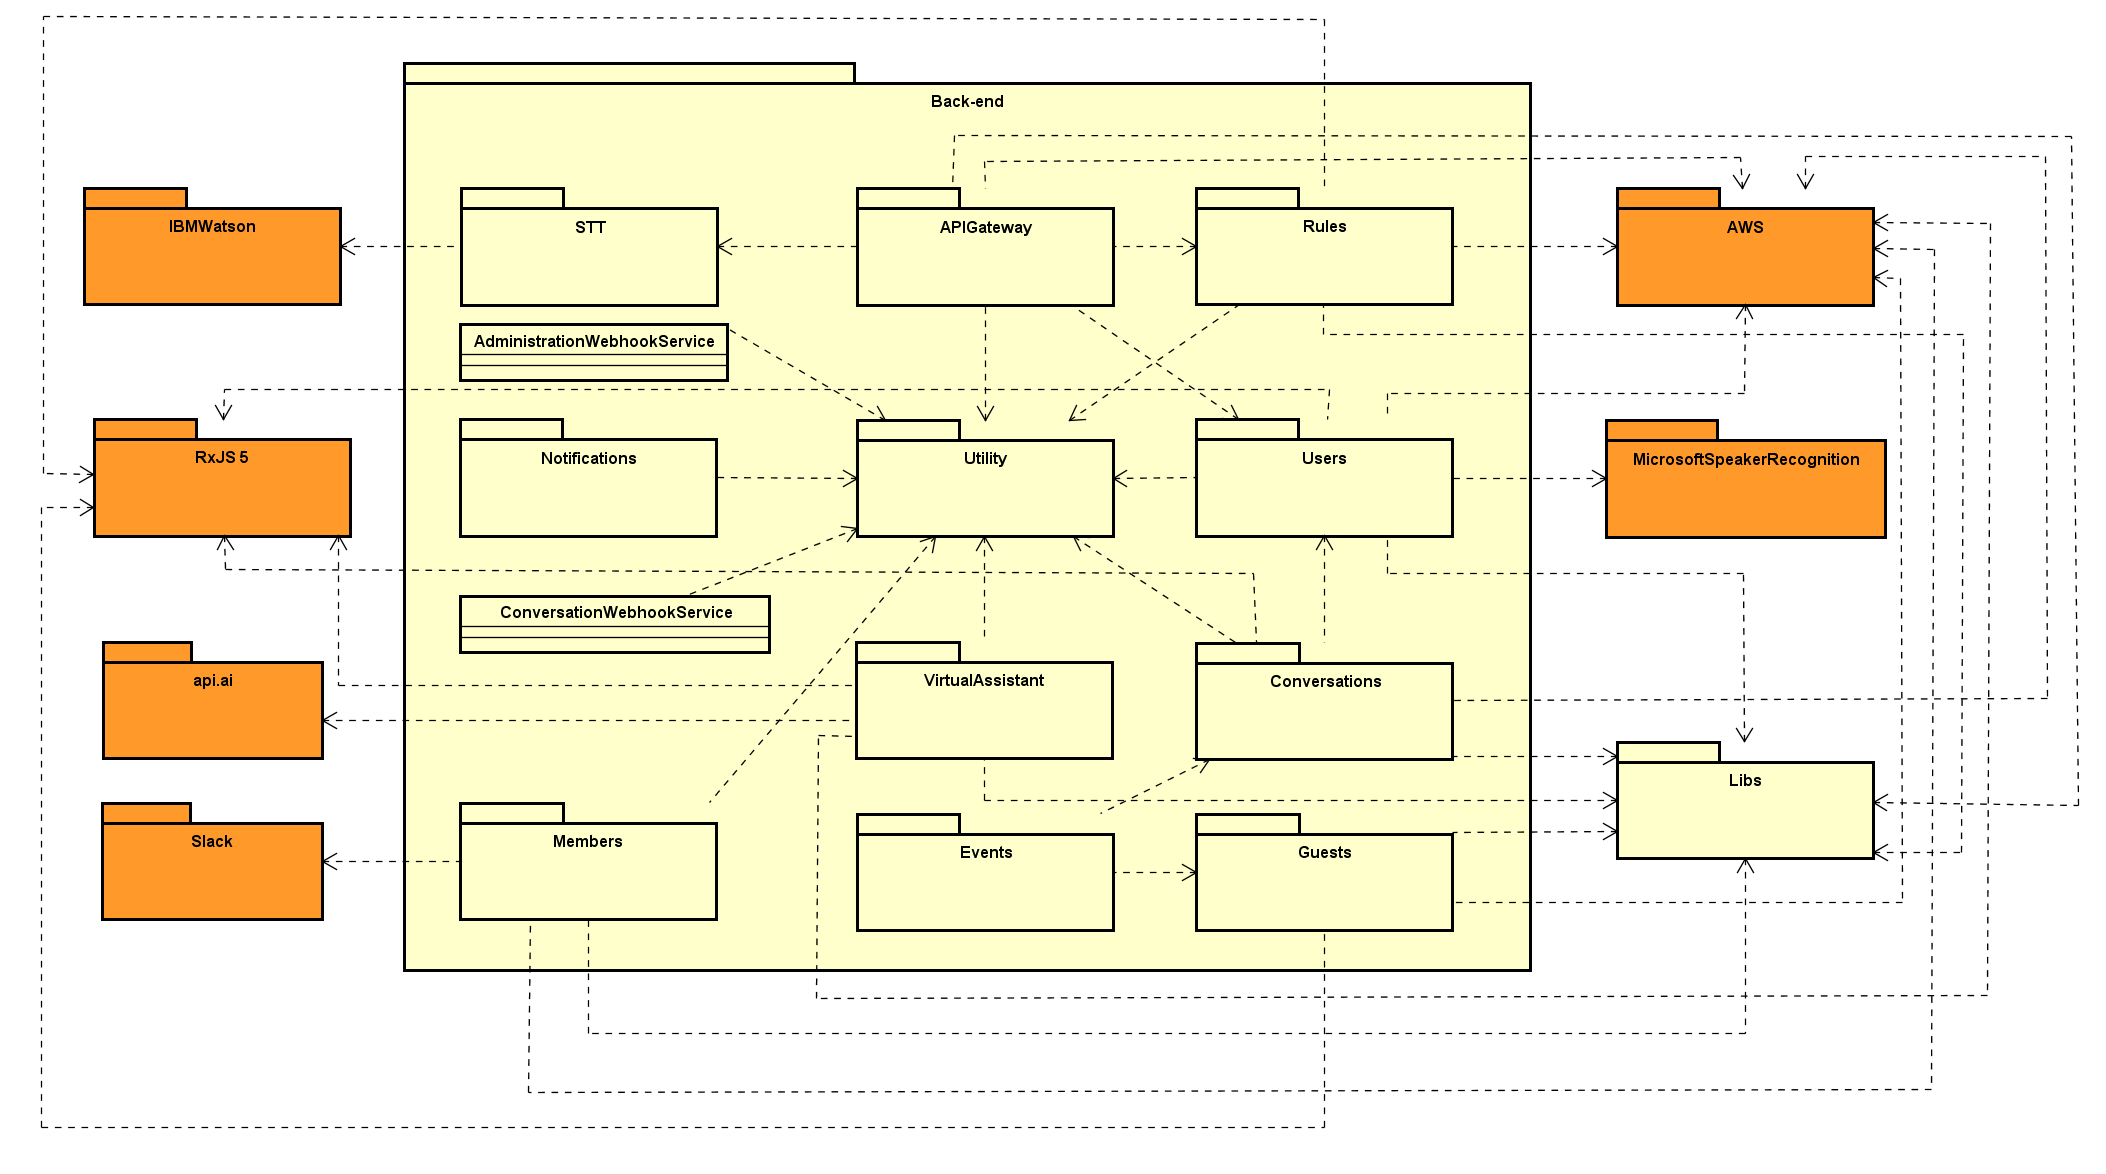
\includegraphics[width=\textwidth,height=\textheight,keepaspectratio]{images/diagrams/back-end/Official_Backend_0304/Back-end.png}
	\caption{Package Back-end}
\end{figure}
\newpage

\subsection{Back-end::\gl{API}\gl{Gateway}}
In questo package sono contenute le classi che realizzano:
\begin{itemize}
	\item le funzionalità da \gl{API Gateway}, permettendo l'interazione \file{Client} - \file{Back-end} tramite la pubblicazione di appositi \gl{endpoint};
	\item la mappatura delle richieste del \file{Client} nelle funzionalità supportate dal \file{Back-end};
	\item la conversione di un audio nel formato accettato dai servizi esterni utilizzati;
	\item la pubblicazione sul topic SNS per notificare la persona desiderata e segnalare la necessità di registrare l'interazione appena avvenuta con l'interlocutore;
	\item il login tramite impronta vocale.
\end{itemize}
\begin{figure}[h] \centering 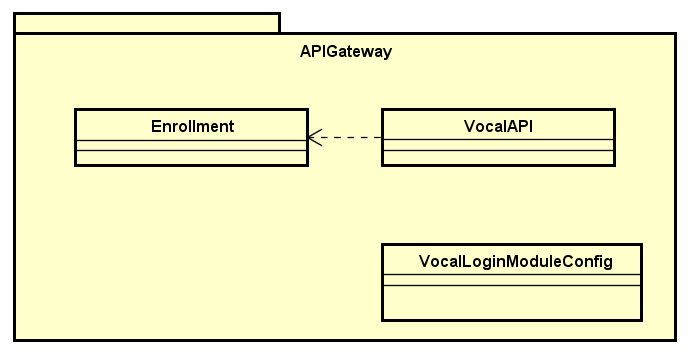
\includegraphics[width=\textwidth,height=\textheight,keepaspectratio]{images/diagrams/back-end/Official_Backend_0304/APIGateway.png}
	\caption{Package Back-end::APIGateway}
\end{figure}
\newpage



\subsection{Back-end::Conversations}
In questo package sono contenute le classi che realizzano: \begin{itemize} \item la definizione di una conversazione e dei messaggi contenuti in essa; \item l'interfaccia per l'interazione con il database contenente le conversazioni sostenute; \item le modalità con le quali i dati devono essere trasmessi dal e al database. \end{itemize}
\begin{figure}[h] \centering 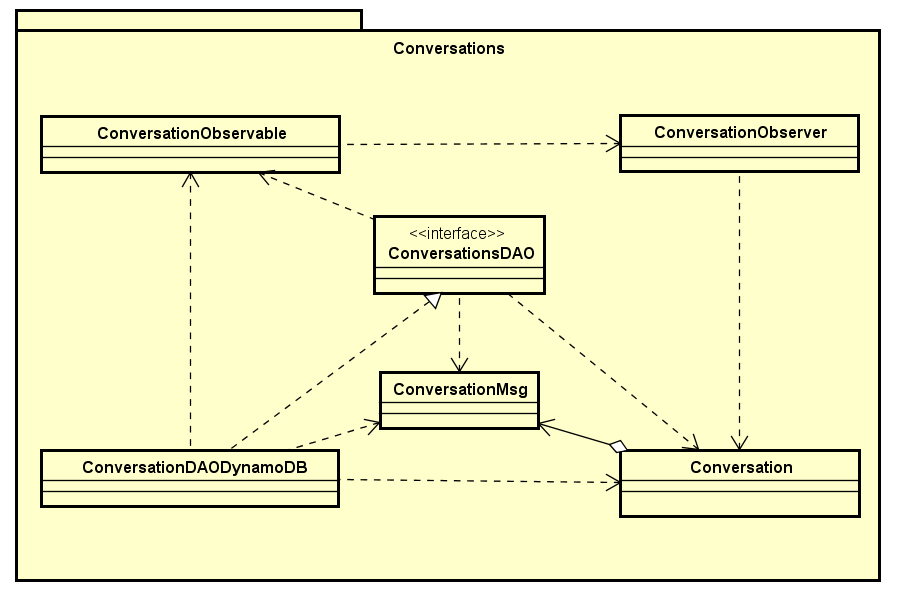
\includegraphics[width=\textwidth,height=\textheight,keepaspectratio]{images/diagrams/back-end/Official_Backend_0304/Conversations.png}
	\caption{Package Back-end::Conversations}
\end{figure}
\newpage

\subsection{Back-end::Events}
In questo package sono contenute le classi che realizzano: \begin{itemize} \item la definizione dei messaggi che devono essere pubblicati sul topic SNS dal quale verranno generati degli eventi; \item la definizione dei dati che le lambda function, innescate da questi eventi, devono processare; \item l'invio di una notifica alla persona desiderata e il salvataggio dell'interazione avvenuta con il \gl{sistema} da parte dell'interlocutore. \end{itemize}
\begin{figure}[h] \centering 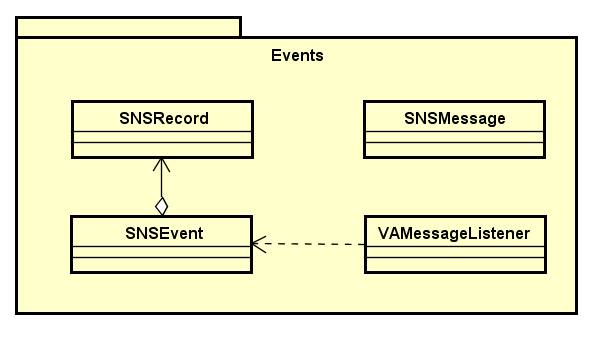
\includegraphics[width=\textwidth,height=\textheight,keepaspectratio]{images/diagrams/back-end/Official_Backend_0304/Events.png}
	\caption{Package Back-end::Events}
\end{figure}
\newpage

\subsection{Back-end::Guests}
In questo package sono contenute le classi che realizzano: \begin{itemize} \item la definizione dei dati associati ad un ospite che ha interagito con il sistema; \item l'interfaccia per l'interazione con il database contenente gli ospiti conosciuti; \item le modalità con le quali i dati devono essere trasmessi dal e al database. \end{itemize}	
\begin{figure}[h] \centering 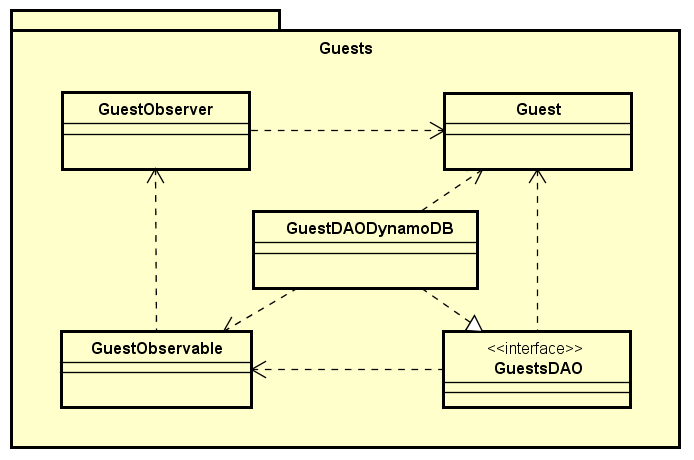
\includegraphics[width=\textwidth,height=\textheight,keepaspectratio]{images/diagrams/back-end/Official_Backend_0304/Guest.png}
	\caption{Package Back-end::Guests}
\end{figure}
\newpage

\subsection{Back-end::Members}
In questo package sono contenute le classi che realizzano: \begin{itemize} \item la definizione dei dati associati ad un membro dell'azienda al quale indirizzare una \gl{direttiva}; \item l'interfaccia per l'interazione con il database contenente i membri dell'azienda; \item le modalità con le quali i dati devono essere trasmessi dal e al database. \end{itemize}
\begin{figure}[h] \centering 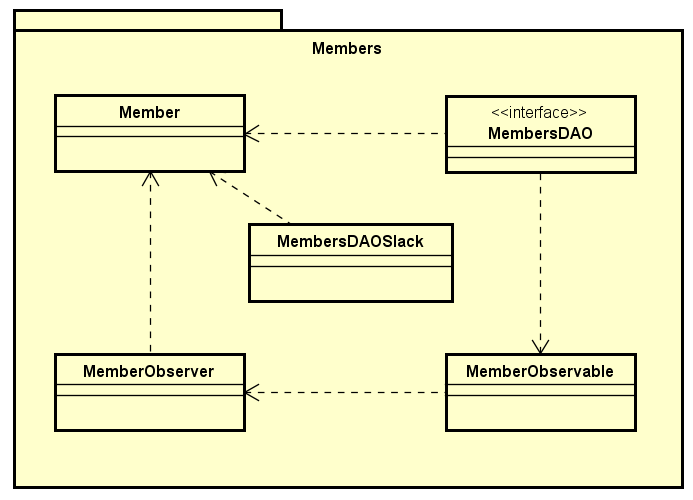
\includegraphics[width=\textwidth,height=\textheight,keepaspectratio]{images/diagrams/back-end/Official_Backend_0304/Member.png}
	\caption{Package Back-end::Members}
\end{figure}
\newpage

\subsection{Back-end::Notifications}
Package contenente le classi e le interfacce che realizzano il \gl{microservizio} relativo alla gestione delle notifiche da inviare alla persona desiderata su una certa piattaforma di messaggistica.\\ Sono contenute le classi che realizzano: \begin{itemize} \item la definizione dei dati di un messaggio da inviare alla persona desiderata; \item la definizione dei dati del canale associato alla persona desiderata; \item il microservizio che espone gli endpoint per permetterne il suo utilizzo. \end{itemize}
\begin{figure}[h] \centering 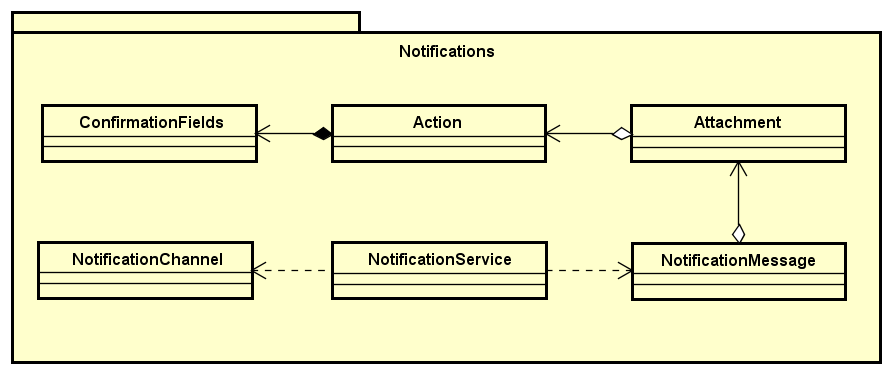
\includegraphics[width=\textwidth,height=\textheight,keepaspectratio]{images/diagrams/back-end/Official_Backend_0304/Notifications.png}
	\caption{Package Back-end::Notifications}
\end{figure}
\newpage

\subsection{Back-end::Rules}
Package contenente le classi e le interfacce che realizzano il microservizio di gestione delle \gl{direttive} per l'assistente virtuale.\\ Vengono offerte funzionalità che permettono: \begin{itemize} \item l'aggiunta di una nuova direttiva; \item l'aggiunta di un nuovo compito (\file{\gl{Task}}) che una direttiva deve eseguire; \item la gestione delle direttive esistenti; \item la gestione dei compiti esistenti. \end{itemize} Sono contenute le classi che realizzano: \begin{itemize} \item la definizione dei dati di una direttiva; \item l'interfaccia per l'interazione con il database contenente le direttive; \item la definizione dei dati di un \gl{task}; \item l'interfaccia per l'interazione con il database contenente i task; \item le modalità con le quali i dati devono essere trasmessi dai e ai database; \item il microservizio che espone gli endpoint per permetterne il suo utilizzo. \end{itemize}
\begin{figure}[h] \centering 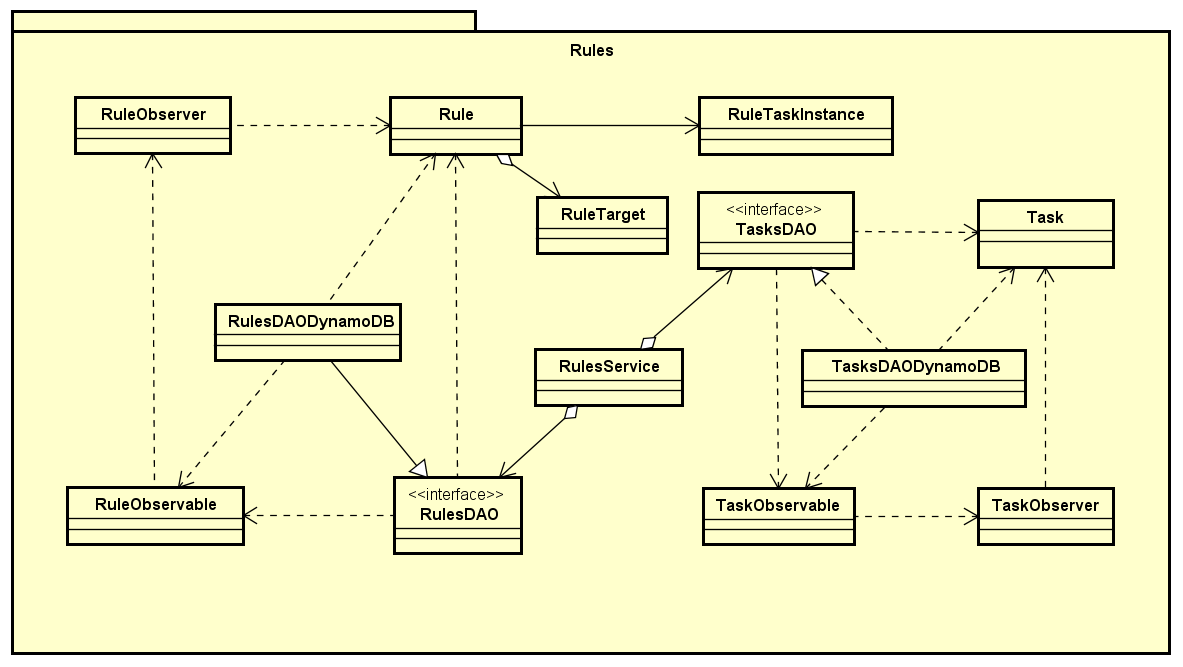
\includegraphics[width=\textwidth,height=\textheight,keepaspectratio]{images/diagrams/back-end/Official_Backend_0304/Rules.png}
	\caption{Package Back-end::Rules}
\end{figure}
\newpage

\subsection{Back-end::STT}
Package che include le classi che si occupano di fornire le funzionalità di \gl{Speech to text}.\\ Le classi contenute realizzano: \begin{itemize} \item l'interfaccia e le modalità di utilizzo del servizio esterno di Speech to Text. \end{itemize}
\begin{figure}[h] \centering 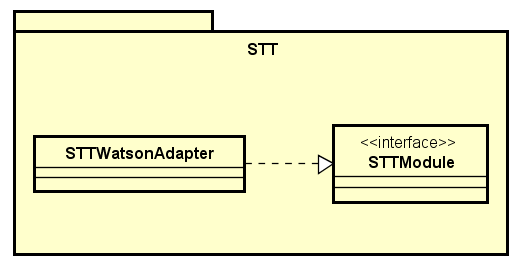
\includegraphics[width=\textwidth,height=\textheight,keepaspectratio]{images/diagrams/back-end/Official_Backend_0304/STT.png}
	\caption{Package Back-end::STT}
\end{figure}
\newpage

\subsection{Back-end::Users}
Package contenente le classi e le interfacce che realizzano il microservizio di autenticazione e registrazione di un amministratore nel sistema.\\ Vengono offerte funzionalità che permettono: \begin{itemize} \item la registrazione di un nuovo amministratore; \item l'autenticazione di un amministratore; \item gestione degli amministratori esistenti. \end{itemize} Sono contenute le classi che realizzano: \begin{itemize} \item la definizione dei dati di un utente registrato; \item l'interfaccia per l'interazione con il database contenente gli utenti registrati; \item le modalità con le quali i dati devono essere trasmessi dal e al database; \item le modalità di interazione che il servizio esterno di riconoscimento vocale; \item il microservizio che espone gli endpoint per permetterne il suo utilizzo. \end{itemize}
\begin{figure}[h] \centering 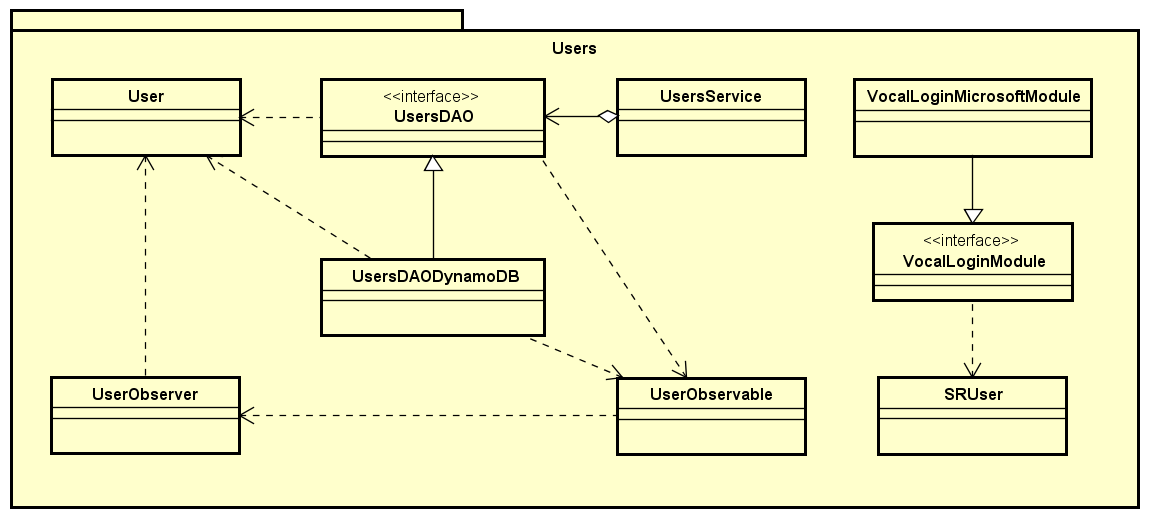
\includegraphics[width=\textwidth,height=\textheight,keepaspectratio]{images/diagrams/back-end/Official_Backend_0304/Users.png}
	\caption{Package Back-end::Users}
\end{figure}
\newpage

\subsection{Back-end::Utility}
Package contenente classi e interfacce, dallo scopo generico, utili ad altri package del back-end
\begin{figure}[h] \centering 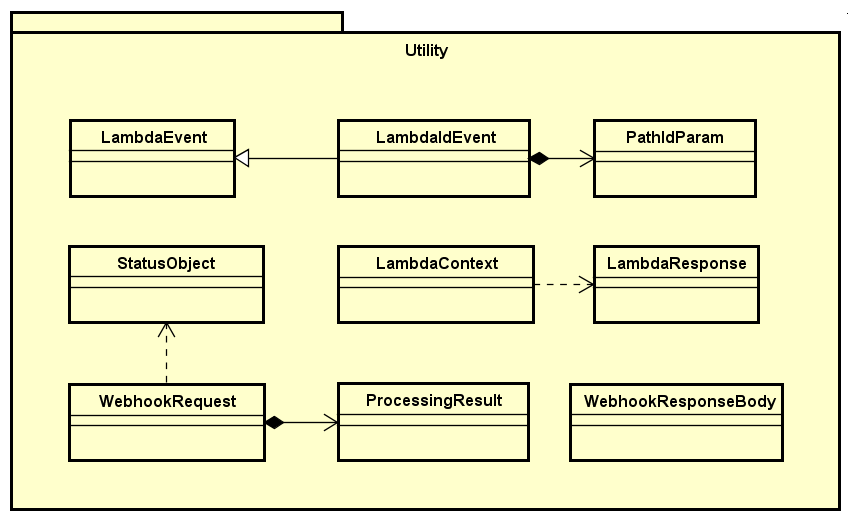
\includegraphics[width=\textwidth,height=\textheight,keepaspectratio]{images/diagrams/back-end/Official_Backend_0304/Utility.png}
	\caption{Package Back-end::Utility}
\end{figure}
\newpage

\subsection{Back-end::VirtualAssistant}
Package contenente le classi e le interfacce che realizzano il microservizio di assistente virtuale .\\ Vengono offerte funzionalità che permettono di: \begin{itemize} \item interrogare l'assistemte virtuale. \end{itemize} Sono contenute le classi che realizzano: \begin{itemize} \item la definizione dei dati di un agent; \item l'interfaccia per l'interazione con il database contenente gli agent; \item le modalità con le quali i dati devono essere trasmessi dal e al database; \item la definizione dei dati da scambiare con i \gl{webhook}; \item l'interfaccia e le modalità di interazione con il servizio esterno di assistente virtuale (api.ai); \item il microservizio che espone gli endpoint per permetterne il suo utilizzo. \end{itemize}
\begin{figure}[h] \centering 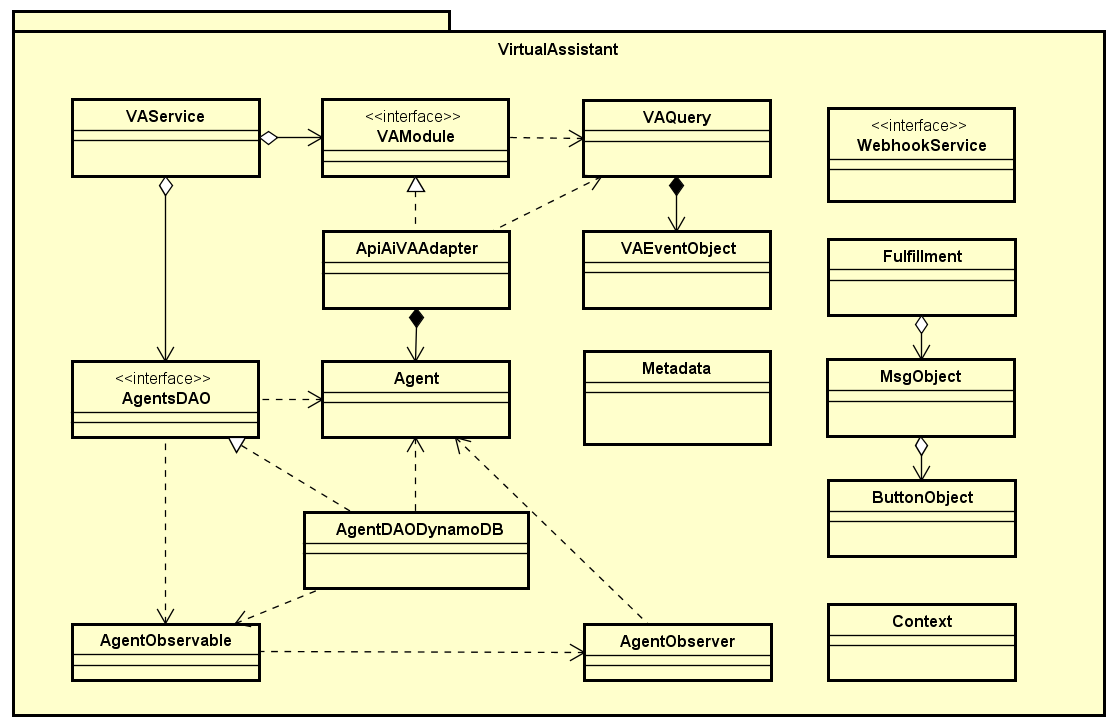
\includegraphics[width=\textwidth,height=\textheight,keepaspectratio]{images/diagrams/back-end/Official_Backend_0304/VirtualAssistant.png}
	\caption{Package Back-end::VirtualAssistant}
\end{figure}
\newpage

\subsection{Client}
Package che racchiude tutte le componenti del client. Il pattern utilizzato per organizzare le componenti è quello di un'architettura \gl{event-driven}.
\begin{figure}[h] \centering 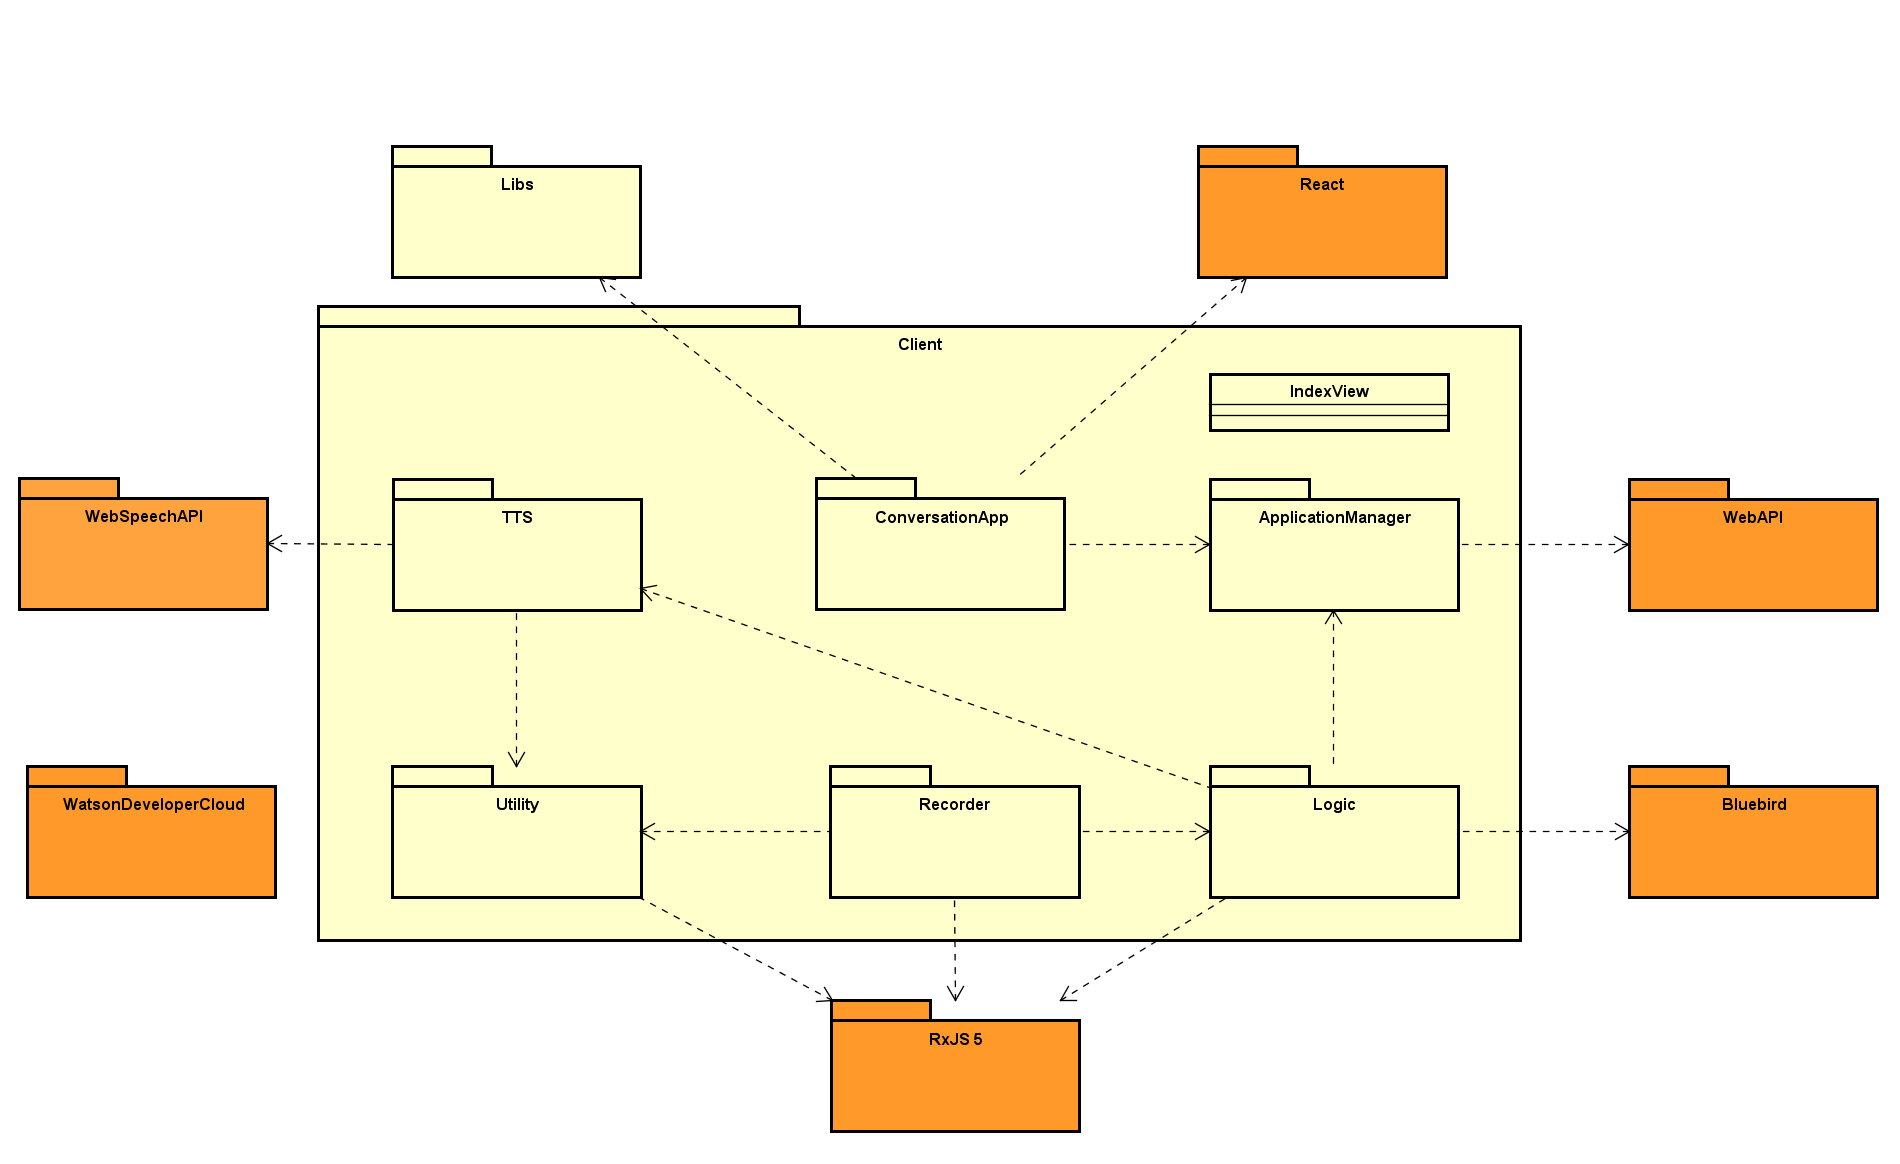
\includegraphics[width=\textwidth,height=\textheight,keepaspectratio]{images/diagrams/client/Client/Client.png}
	\caption{Package Client}
\end{figure}
\newpage


\subsection{Client::ApplicationManager}
Package contenente le classi che si occupano della gestione delle applicazioni con le quali l'utente può interagire.\\ Vengono offerte funzionalità che permettono: \begin{itemize} \item la reazione a dei dati di risposta arrivati dal \file{Back-end}; \item la definizione di ciò che va a comporre una applicazione; \item il salvataggio dello stato di un'applicazione; \item il cambio di un'applicazione con un'altra. \end{itemize}
\begin{figure}[h] \centering 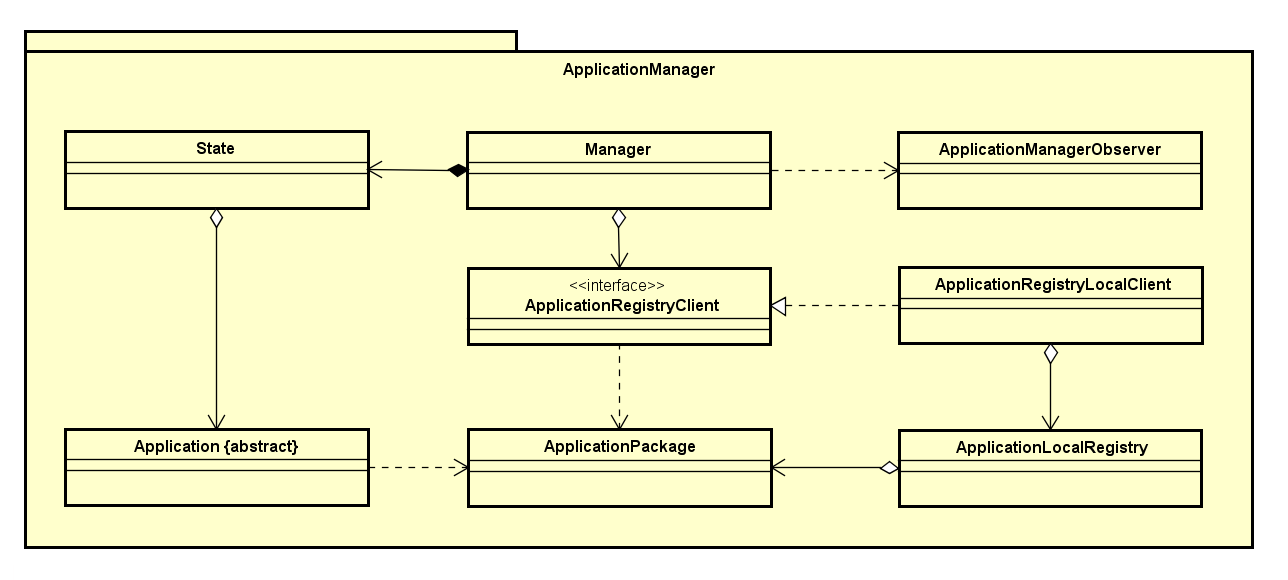
\includegraphics[width=\textwidth,height=\textheight,keepaspectratio]{images/diagrams/client/Client/ApplicationManager.png}
	\caption{Package Client::ApplicationManager}
\end{figure}
\newpage

\subsection{Client::ConversationApp}
In questo package è definita l'applicazione di conversazione, la quale fornisce un'interfaccia utente per l'interazione con l'assistente virtuale.\\ Le classi contenute in questo package permettono di: \begin{itemize} \item tenere traccia delle conversazioni effettuate con gli ospiti; \item notificare gli observer collegati che è stata decisa la \file{ConversationAction}; \item gestire i comandi da eseguire da \file{ConversationApp}. \end{itemize}
\begin{figure}[h] \centering 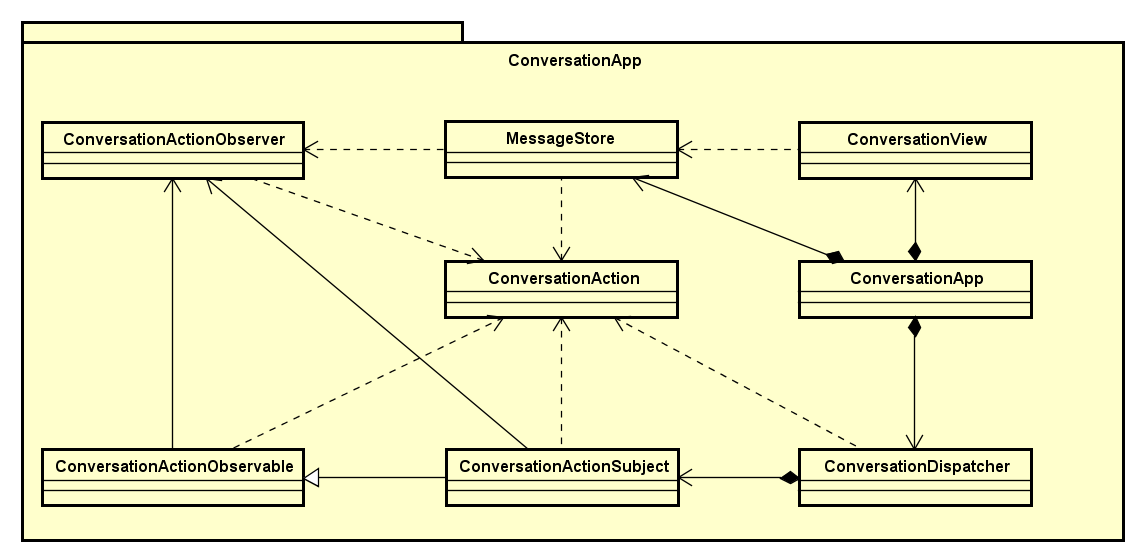
\includegraphics[width=\textwidth,height=\textheight,keepaspectratio]{images/diagrams/client/Client/ConversationApp.png}
	\caption{Package Client::ConversationApp}
\end{figure}
\newpage

\subsection{Client::Logic}
Package contenente le classi che gestiscono la logica del client e che si occupano della comunicazione con il back-end.\\ Le classi contenute permettono : \begin{itemize} \item l'esecuzione una determinata azione in base ai dati arrivati come richiesta dal registratore vocale; \item il notificare alle classi interessate l'arrivo del testo di risposta dal \file{Back-end}; \item l'esecuzione di richieste \gl{HTTP} sostituendo le funzioni di \gl{Callback} fornite da Javascript con le Promise che sono più chiare in casi di annidamento; \end{itemize}
\begin{figure}[h] \centering 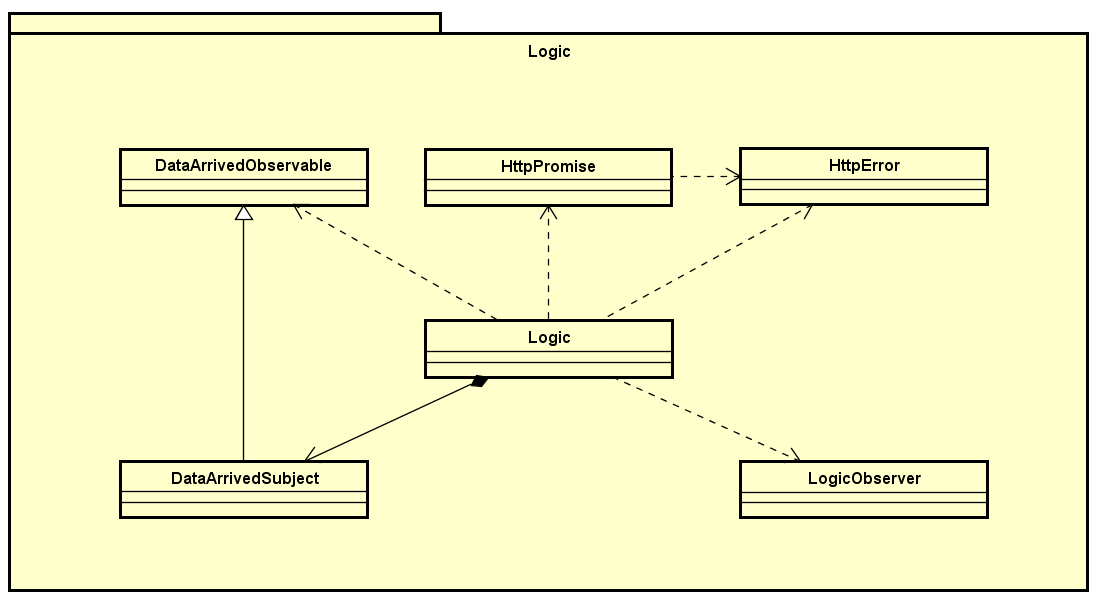
\includegraphics[width=\textwidth,height=\textheight,keepaspectratio]{images/diagrams/client/Client/Logic.png}
	\caption{Package Client::Logic}
\end{figure}
\newpage


\subsection{Client::Recorder}
Package contenente le componenti che realizzano il \gl{text to speech}. Vengono offerte funzionalità che permettono: \begin{itemize} \item la reazione a dei dati arrivati come riposta dal \file{Back-end}; \item la riproduzione audio del testo fornito come risposta dall'assistente virtuale. \end{itemize}
\begin{figure}[h] \centering 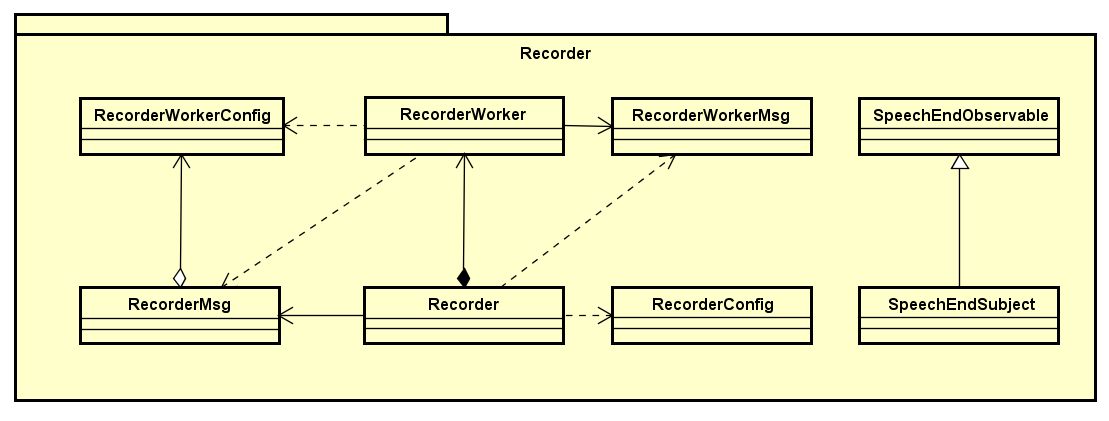
\includegraphics[width=\textwidth,height=\textheight,keepaspectratio]{images/diagrams/client/Client/Recorder.png}
	\caption{Package Client::Recorder}
\end{figure}
\newpage


\subsection{Client::TTS}
Package contenente le componenti che realizzano il text to speech. Vengono offerte funzionalità che permettono: \begin{itemize} \item la reazione a dei dati arrivati come riposta dal \file{Back-end}; \item la riproduzione audio del testo fornito come risposta dall'assistente virtuale. \end{itemize}
\begin{figure}[h] \centering 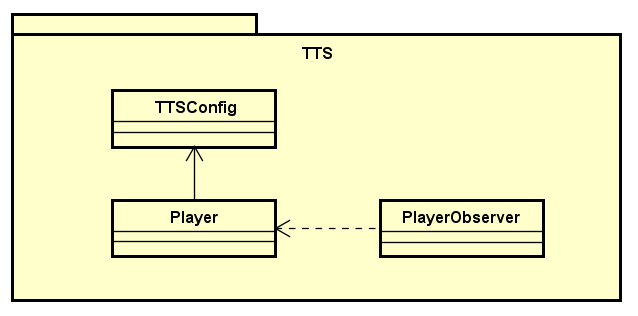
\includegraphics[width=\textwidth,height=\textheight,keepaspectratio]{images/diagrams/client/Client/TTS.png}
	\caption{Package Client::TTS}
\end{figure}
\newpage


\subsection{Client::Utility}
Package contenente classi e interfacce, dallo scopo generico, utili ad altri package del client.
\begin{figure}[h] \centering 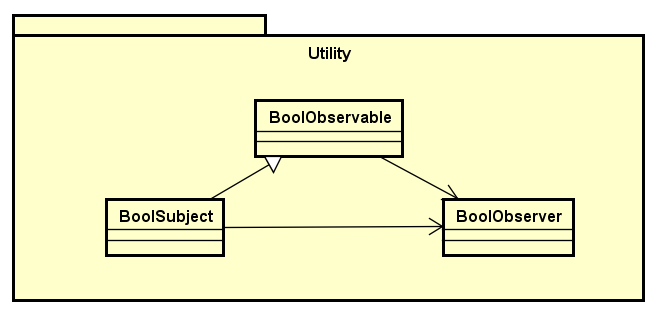
\includegraphics[width=\textwidth,height=\textheight,keepaspectratio]{images/diagrams/client/Client/Utility.png}
	\caption{Package Client::Utility}
\end{figure}
\newpage